\chapter{Digital Image Processing}

We worked with images from
CRIC Database.
% TODO Add citation
The 400 images
have \(1376~\times~1020\)~pixels.

\begin{figure}
  \centering
  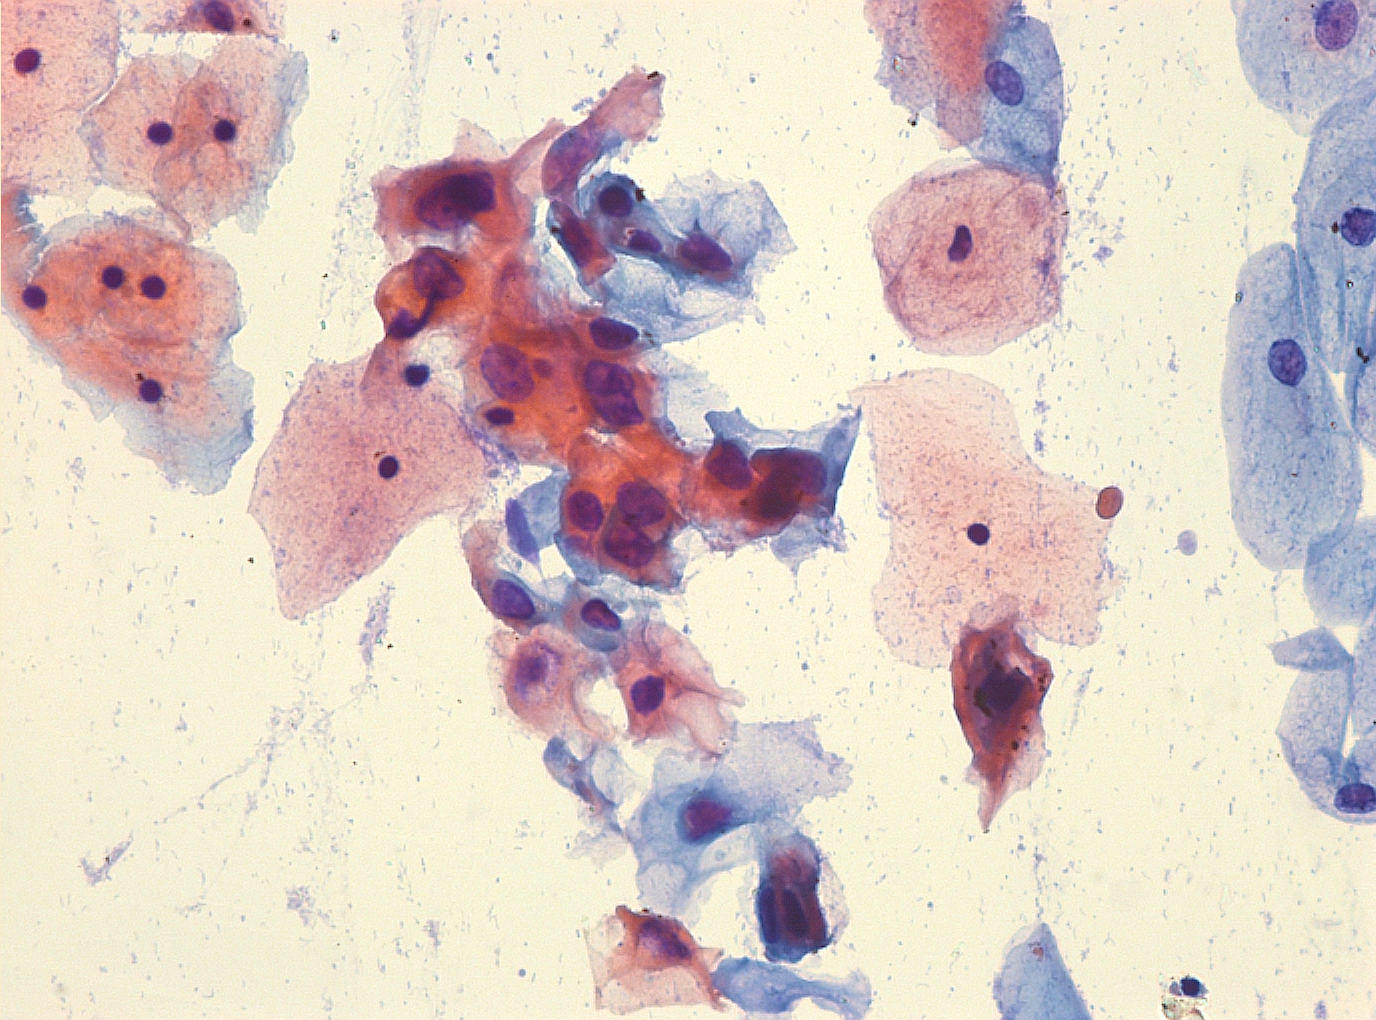
\includegraphics{R/img/be340ee72689dfe3f8dc9c24de6127f4.png}
  \caption{Example of image from CRIC}
  % TODO Add DOI
\end{figure}

We store the image as 3-D array \(A\),
containing
\(M\) rows,
\(N\) columns,
and
3 channels
(red, green, and blue).
For clarity
and
convenience,
since we used Python as programming language,
we use integer values for the discrete coordinates:
\(x = 0, 1, 2, \ldots, M - 1\),
\(y = 0, 1, 2, \ldots, N - 1\),
\(z = 0, 1, 2\).
\(x\), \(y\), and \(z\)
are referred as spatial variables.

The value \(a_{x, y, z}\)
is referred as intensity of \(A\)
at \(x\), \(y\), and \(z\)
and they are integers
in the interval
\([0, 255]\).

A pixel \(p\)
at coordinates \((x, y, z\)
has four horizontal and vertical neighbours,
denoted by \(N_4(p)\):
\begin{itemize}
\item \(x - 1, y, z\)
\item \(x + 1, y, z\)
\item \(x, y - 1, z\)
\item \(x, y + 1, z\)
\end{itemize}
It also has for diagonal neighbours,
denoted by \(N_D(p)\):
\begin{itemize}
\item \(x - 1, y - 1, z\)
\item \(x + 1, y - 1, z\)
\item \(x + 1, y + 1, z\)
\item \(x - 1, y + 1, z\)
\end{itemize}
The \(N_4(p) \cup N_D(p)\)
is called 8-neighbours of \(p\)
and denoted by \(N_8(p)\).

%%% Local Variables:
%%% mode: latex
%%% TeX-master: "masters_dissertation"
%%% End:
